\section{Oscilador em Anel}
O oscilador em anel é uma topologia de circuito muito utilizada para a caracterização de parâmetros de circuito de diversos tipos. Um dos principais motivos para isso é a capacidade de representar uma aplicação operando em alta velocidade. Segundo \cite{Bhushan} medidas feitas sob estas condições são mais próximas das aplicações reais da tecnologia do que parametrização dc convencionais, o que é verdade principalmente para dispositivos CMOS de alta performance.

Eles também são utilizados como sensores de alta precisão que aumentam a confiabilidade de um chip, podendo ser usado para monitorar diversos parâmetros como variações de processo, temperatura e efeitos de envelhecimento \cite{Sato}. Podem ser facilmente implementados e possuem um consumo de energia pequeno.

O circuito do oscilador em anel consiste em portas lógicas inversoras ligadas em sequência com uma realimentação entre a saída da última e a entrada da primeiro. É necessário que haja um número ímpar de inversores, para assim haver uma inversão periódica da entrada e da saída. O atraso de propagação de cada inversor e a realimentação gera uma onda quadrada na saída.

O período da oscilação é duas vezes o somatório do atraso de cada inversor. A Equação \ref{eq:TotalDelay} mostra frequência de oscilação, considerando que todos os inversores têm o mesmo atraso, onde N representa o número de inversores e Ta representa o tempo de atraso de um inversor.

\begin{equation}
    F = \frac{1}{2.N.Ta}
    \label{eq:TotalDelay}
\end{equation}
         
A Figura \ref{fig:RingOsc} mostra o diagrama do oscilador em anel. O circuito em questão também possui um sinal de \textit{enable}, que, além de servir para controlar o funcionamento do oscilador, também evita que o circuito entre em um estado de metaestabilidade e não oscile.

\begin{figure}[H]
    \centering
    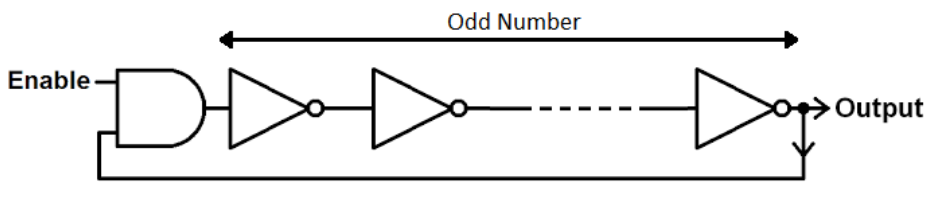
\includegraphics[width=\linewidth]{figures/ReferencialTeorico/RingOscModified.png}
    \caption{Oscilador em Anel. Fonte: \cite{Sparkfun}, modificado pelo autor}
    \label{fig:RingOsc}
\end{figure}

Uma quantidade na casa das centenas de inversores no circuito reduzirá as variações aleatórias intrínsecas de cada MOSFET que poderiam aparecer caso fossem medidos individualmente, permitindo uma caracterização mais confiável e robusta.

O trabalho de \cite{Bhushan} descreve estratégias de design para estruturas de osciladores em anel e também apresenta o uso dessas estruturas para mensurar consumo de energia e outros parâmetros de MOSFETs.

Um outro trabalho, \cite{Michal} realizou estudos para reduzir o consumo de energia de osciladores em anel, conseguindo isso reduzindo o número de inversores, mas acoplando capacitores a cada um deles para aumentar o atraso.